% Chapter 2
\chapter{Tecnologias Emergentes para a Monitorização e Previsão do Estado Fisiológico}

\label{chap:TecnologiasEmergentes}

\section{Metodologia de Pesquisa}
\label{sec:metodologia}

A presente revisão sistemática foi concebida com o objetivo de identificar e analisar a literatura científica mais relevante sobre tecnologias emergentes para a monitorização fisiológica, focando-se na previsão de estados humanos mediante técnicas de inteligência artificial e aprendizagem automática.

Para garantir o rigor e a reprodutibilidade do estudo, foi adotada a \textbf{metodologia PRISMA} (Preferred Reporting Items for Systematic Reviews and Meta-Analyses), que fornece um quadro estruturado para o planeamento, a execução e a apresentação de revisões sistemáticas. Esta abordagem permite documentar de forma transparente o processo de pesquisa, seleção, extração e síntese da informação, assegurando que os resultados obtidos sejam objetivos e comparáveis. Esta opção metodológica é igualmente adotada em revisões recentes, como a de Ribeiro, R., Martinho, D. et al.~\cite{ribeiro2026wearable}, sobre a utilização de dispositivos vestíveis na monitorização remota da saúde.

A revisão tem um alcance temporal dos últimos cinco anos (2020–2025), considerando estudos que apresentam aplicações reais ou experimentais de monitorização fisiológica mediante sensores portáteis e modelos preditivos. A análise centra-se em identificar tendências, técnicas e aplicações práticas relevantes, bem como desafios e limitações reportados na literatura.

A abordagem metodológica adotada inclui as seguintes fases principais: definição de perguntas principais e secundárias de investigação, identificação de fontes de informação e bases de dados académicas pertinentes, construção de estratégias de pesquisa, seleção de estudos relevantes segundo critérios de inclusão e exclusão pré-definidos, extração sistemática de dados e síntese de resultados. Este processo estruturado garante que a revisão proporcione um estado da arte sólido e fundamentado, que servirá como base para a posterior discussão e desenvolvimento do sistema de previsão do estado fisiológico no contexto do gémeo digital humano.

Cabe destacar que a metodologia e os resultados desta revisão sistemática foram também consolidados num artigo científico intitulado ``\textit{A Review of Physiological Monitoring and Prediction in Workers in High-Risk Construction Environments}''~\cite{freitas2026physiological}. O artigo foi aceite e apresentado na conferência INISTA 2026~\cite{inista2026}, constituindo um resultado de disseminação científica do processo de revisão da literatura apresentado neste capítulo.


\section{Questões de Pesquisa}
\label{sec:questoes}

A presente revisão sistemática tem como objetivo analisar o estado da arte em tecnologias e modelos de inteligência artificial aplicados à monitorização fisiológica, com especial ênfase na interpretação e previsão do estado humano em ambientes de alto risco. Para orientar o processo de pesquisa e análise da literatura, foram definidas as seguintes questões de investigação.

\textbf{Pergunta principal}

QP1: Que tecnologias e modelos de inteligência artificial são atualmente empregues para a monitorização, interpretação e previsão do estado fisiológico de trabalhadores ou indivíduos em ambientes de alto risco, a partir de dados obtidos mediante sensores portáteis?

\textbf{Perguntas secundárias}

\begin{table}[H]
\caption{Perguntas secundárias}
\label{tab:preguntas}
\centering
\renewcommand{\arraystretch}{1.5}
\begin{tabular}{c p{12cm}}
\toprule
\tabhead{ID} & \tabhead{Pergunta} \\
\midrule
QS1 & Que tipos de sinais fisiológicos são habitualmente recolhidos e utilizados na literatura para a monitorização do estado humano (HR, HRV, respiração, EEG, etc.)? \\
QS2 & Que técnicas de aprendizagem automática e aprendizagem profunda são aplicadas com maior frequência para a análise e a previsão de estados como stress, fadiga, carga fisiológica ou nível de atenção? \\
QS3 & Que arquiteturas e modelos são utilizados para a análise de séries temporais fisiológicas e quais são as suas principais vantagens e limitações? \\
QS4 & Quais são as métricas de avaliação mais utilizadas para validar o desempenho dos modelos propostos em estudos de monitorização fisiológica? \\
QS5 & Que limitações e desafios são identificados na literatura para a implementação de sistemas de previsão do estado humano em tempo real? \\
QS6 & Que mecanismos de comunicação, notificação ou retroalimentação ao utilizador são descritos na literatura? \\
\bottomrule
\end{tabular}
\end{table}

\section{Fontes de Literatura Científica}
\label{sec:bases}

Com o objetivo de garantir uma revisão sistemática completa e representativa do estado atual da investigação, foram selecionadas três bases de dados académicas amplamente reconhecidas pela sua relevância nas áreas de inteligência artificial, engenharia biomédica e ciências da saúde. Estas bases de dados permitem aceder a literatura científica revista por pares e de alto impacto, alinhada com os objetivos desta tese.

\begin{table}[H]
\caption{Bases de dados utilizadas na revisão sistemática}
\label{tab:bases}
\centering
\begin{tabular}{c l l}
\toprule
\tabhead{ID} & \tabhead{Database} & \tabhead{URL} \\
\midrule
D1 & PubMed & \url{https://pubmed.ncbi.nlm.nih.gov} \\
D2 & IEEE Xplore & \url{https://ieeexplore.ieee.org} \\
D3 & ScienceDirect & \url{https://www.sciencedirect.com} \\
D4 & MDPI & \url{https://www.mdpi.com} \\
\bottomrule
\end{tabular}
\end{table}

O PubMed foi selecionado pela sua especialização em ciências da saúde e medicina, proporcionando acesso a estudos relacionados com a monitorização fisiológica, bio-sinais e aplicações de sensores portáteis para a avaliação do estado humano. Esta base de dados é especialmente relevante para compreender o contexto fisiológico e biomédico dos sinais analisados.

O IEEE Xplore foi incluído devido ao seu forte enfoque em engenharia, informática e tecnologias emergentes. Esta base de dados oferece uma ampla coleção de trabalhos sobre inteligência artificial, aprendizagem automática, processamento de sinais e sistemas de monitorização em tempo real, aspetos chave para o desenvolvimento de modelos preditivos baseados em dados fisiológicos.

O ScienceDirect foi considerado pela sua cobertura em engenharia biomédica, saúde digital e análise de sinais, incluindo revistas de alto impacto relacionadas com sensores, dispositivos portáteis e aplicações de inteligência artificial em contextos de monitorização fisiológica.

O MDPI (Multidisciplinary Digital Publishing Institute), uma editora académica de acesso aberto, foi incluído como fonte complementar devido à relevância das suas revistas nas áreas de inteligência artificial, engenharia biomédica, sensores e análise de sinais fisiológicos. A pesquisa nesta plataforma permitiu identificar estudos recentes sobre técnicas de clustering e aprendizagem automática aplicadas à monitorização fisiológica.

A combinação destas fontes de literatura garante um equilíbrio adequado entre literatura técnica e biomédica, contribuindo para uma revisão sistemática robusta e alinhada com o alcance da presente investigação.

\section{Termos de Pesquisa}
\label{sec:termos}

Os termos de pesquisa foram definidos a partir das questões de investigação colocadas, com o objetivo de identificar estudos relevantes relacionados com a monitorização fisiológica baseada em sensores portáteis e o uso de técnicas de inteligência artificial para a interpretação e previsão do estado humano. Para garantir uma pesquisa estruturada e reprodutível, os termos foram organizados em diferentes \textit{âmbitos} temáticos que refletem os principais eixos desta revisão sistemática: sinais fisiológicos, tecnologias de sensorização, técnicas de inteligência artificial e contexto de aplicação.

\begin{table}[H]
\caption{Termos de pesquisa por âmbito temático}
\label{tab:termos}
\centering
\footnotesize
\begin{tabular}{p{3cm} p{11cm}}
\toprule
\tabhead{Âmbito} & \tabhead{Cadeia de pesquisa} \\
\midrule
Sinais Fisiológicos e Cognitivos & ("physiological signals" OR "heart rate" OR "HRV" OR "respiration" OR "EEG") \\
\addlinespace
Sensores Portáteis & ("wearable sensors" OR "wearable devices" OR "smartwatch" OR "chest strap" OR "physiological monitoring") \\
\addlinespace
Técnicas de Inteligência Artificial & ("AI" OR "artificial intelligence" OR "machine learning" OR "deep learning" OR "neural networks" OR "time series analysis" OR "digital twin" OR "clustering") \\
\addlinespace
Previsão do Estado Humano & ("stress" OR "fatigue" OR "attention" OR "human state") \\
\addlinespace
Notificações e Alertas & ("alerts" OR "warnings" OR "notifications" OR "feedback") \\
\addlinespace
Contextos de Alto Risco & ("worker safety" OR "human safety" OR "workplace monitoring" OR "industrial environments") \\
\bottomrule
\end{tabular}
\end{table}

A combinação destes âmbitos permitiu construir cadeias de pesquisa adaptadas a cada base de dados, maximizando a cobertura de estudos relevantes e reduzindo a inclusão de trabalhos fora do alcance da investigação.

\begin{itemize}
\item O âmbito relacionado com \textbf{sinais fisiológicos} foi incluído para capturar os distintos tipos de variáveis biométricas empregues na monitorização do estado humano.
\item O âmbito dos \textbf{sensores portáteis} permitiu identificar estudos baseados em dispositivos de aquisição de dados em contextos reais e não invasivos.
\item O âmbito das \textbf{técnicas de inteligência artificial} foi definido para abranger tanto abordagens clássicas como métodos avançados de aprendizagem profunda aplicados à análise de dados fisiológicos.
\item O âmbito da \textbf{previsão do estado humano} centrou-se nos objetivos finais dos sistemas analisados, como a deteção de stress, fadiga ou carga cognitiva.
\item O âmbito das \textbf{notificações e alertas} foi incorporado para identificar como os sistemas comunicam a informação gerada ao utilizador final.
\item Finalmente, o âmbito relativo a \textbf{contextos de alto risco} permitiu contextualizar os estudos em cenários onde a monitorização em tempo real tem um impacto direto na segurança e no desempenho humano.
\end{itemize}

\section{Critérios de Inclusão e Exclusão}
\label{sec:criterios}

Os critérios de inclusão e exclusão foram definidos com o objetivo de garantir a seleção de estudos relevantes, coerentes com as questões de investigação e o alcance desta revisão sistemática. Estes critérios permitiram filtrar trabalhos que abordam a monitorização fisiológica mediante sensores portáteis e a aplicação de técnicas de inteligência artificial para a interpretação e previsão do estado humano, excluindo estudos fora deste contexto.

\newpage
Foram incluídos estudos que cumprissem pelo menos um dos seguintes critérios:

\begin{table}[H]
\caption{Critérios de inclusão}
\label{tab:inclusion}
\centering
\begin{tabular}{c p{12cm}}
\toprule
\tabhead{ID} & \tabhead{Critério de Inclusão} \\
\midrule
IC1 & Estudos que utilizem sinais fisiológicos adquiridos mediante sensores portáteis ou dispositivos. \\
IC2 & Trabalhos que apliquem técnicas de IA de aprendizagem automática ou aprendizagem profunda para a interpretação, classificação ou previsão do estado humano. \\
IC3 & Estudos orientados à monitorização de estados fisiológicos, como stress, fadiga, carga fisiológica ou nível de atenção. \\
IC4 & Investigações aplicadas a ambientes laborais, industriais, de alto risco ou contextos comparáveis com monitorização contínua. \\
IC5 & Estudos que descrevam ou implementem mecanismos de comunicação, interface ou sistemas de notificação e alertas para o utilizador final. \\
\bottomrule
\end{tabular}
\end{table}

Foram excluídos estudos que cumprissem algum dos seguintes critérios:

\begin{table}[H]
\centering
\caption{Critérios de exclusão}
\label{tab:exclusion}
\begin{tabular}{c p{12cm}}
\toprule
\tabhead{ID} & \tabhead{Critério de exclusão} \\
\midrule
EC1 & Publicações não redigidas em inglês. \\
EC2 & Estudos publicados antes do ano 2020. \\
EC3 & Publicações que não tenham sido revistas por pares, incluindo artigos de opinião, resumos, pósteres, patentes ou livros. \\
EC4 & Estudos duplicados. \\
EC5 & Estudos que não utilizem dados fisiológicos reais ou que se baseiem exclusivamente em dados simulados sem validação. \\
EC6 & Trabalhos centrados unicamente no design de hardware ou sensores, sem análise do estado fisiológico mediante modelos de IA. \\
\bottomrule
\end{tabular}
\end{table}

\section{Diagrama PRISMA}
\label{sec:prisma}

O processo de seleção de estudos foi realizado seguindo as diretrizes do modelo PRISMA (Preferred Reporting Items for Systematic Reviews and Meta-Analyses), com o objetivo de garantir transparência, reprodutibilidade e rigor metodológico na revisão sistemática.

Na fase de \textbf{identificação}, foram localizados os estudos potencialmente relevantes mediante as cadeias de pesquisa definidas nas bases de dados selecionadas. No total, foram localizados 128 registos através das pesquisas no Science Direct (n = 57), IEEE Xplore (n = 59), PubMed (n = 8) e MDPI (n = 4). Posteriormente, foram eliminados os duplicados, confirmando que todos os registos eram únicos (n = 128).

Durante a fase de \textbf{crivo}, foram avaliados os títulos e resumos dos estudos, resultando na exclusão de 64 registos que não eram relevantes ou não estavam alinhados com o tema de investigação.

Na fase de \textbf{elegibilidade}, foram analisados os textos completos de 64 artigos para determinar a sua adequação ao alcance da revisão. Após a aplicação de critérios específicos (EC1, EC2, EC3, EC4, EC5, EC6, IC1, IC2, IC3, IC4, IC5), foram excluídos 23 estudos que não cumpriam os critérios estabelecidos.

Finalmente, a fase de \textbf{inclusão} contemplou 41 estudos que cumpriram todos os critérios de seleção e foram incorporados à análise qualitativa dos resultados.

O diagrama PRISMA que acompanha esta secção (\ref{fig:prisma}) ilustra de forma estruturada cada uma destas fases, apresentando claramente o fluxo de identificação, triagem, elegibilidade e inclusão dos estudos.

\begin{figure}[H]
\centering
\includegraphics[width=0.7\textwidth]{ch2/assets/prisma.png}
\caption{Diagrama PRISMA}
\label{fig:prisma}
\end{figure}

\section{Avaliação de qualidade dos estudos adquiridos}
\label{sec:evaluacion}

Para complementar a revisão sistemática, foi elaborada uma tabela de avaliação (Tabela \ref{tab:evaluacion}) com o objetivo de priorizar os estudos mais relevantes para os objetivos desta tese. Esta etapa assume particular importância visto que, dada a natureza multidisciplinar do tema, é pouco frequente que um único estudo aborde simultaneamente todas as dimensões da presente investigação (sensores portáteis, dados fisiológicos, modelos de IA, contextos de risco e mecanismos de alerta).

Desta forma, o processo de avaliação de qualidade surge como uma ferramenta metodológica necessária para destacar os trabalhos que melhor se enquadram no âmbito desta revisão, que se centra no desenvolvimento de um módulo preditivo baseado em gémeos digitais humanos para a previsão de estados fisiológicos em trabalhadores da construção. Cada estudo foi pontuado segundo quatro critérios chave: cada resposta afirmativa recebia um ponto, enquanto que as negativas não pontuavam, atribuindo-se 0.5 em casos intermédios ou parciais. Este ranking permitiu identificar os estudos com maior afinidade técnica, orientando a seleção de estratégias e arquiteturas a implementar no sistema final.

\begin{table}[H]
\caption{Perguntas de qualidade}
\label{tab:evaluacion}
\centering
\begin{tabular}{l p{10cm} l}
\toprule
QA & Pergunta & Pontuação \\
\midrule
QA1 & O estudo utiliza sinais fisiológicos adquiridos mediante sensores portáteis ou dispositivos. & Sim (+1); Não (0) \\
QA2 & Aplicam-se técnicas de IA de ML ou DL para interpretação, classificação ou previsão. & Sim (+1); Não (0) \\
QA3 & O estudo monitoriza ou prevê estados fisiológicos como stress, fadiga, carga fisiológica ou atenção. & Sim (+1); Não (0) \\
QA4 & A investigação aplica-se a ambientes de obra, ou ambientes de alto risco ou comparáveis. & Sim (+1); Não (0) \\
\bottomrule
\end{tabular}
\end{table}

Com o objetivo de estabelecer uma base sólida para a entrega preliminar do presente trabalho, a exploração dos resultados e a resposta às perguntas de investigação centram-se especificamente no subconjunto de 14 artigos científicos que obtiveram a classificação máxima de 4 valores. Estes estudos foram selecionados como o núcleo central desta revisão por apresentarem um alinhamento total com os pilares técnicos e contextuais da tese.

Os restantes estudos integrados na revisão sistemática (com pontuações inferiores a 4) são utilizados como referencial de apoio, servindo para contextualizar tendências gerais, validar discussões específicas ou fornecer exemplos de abordagens complementares na literatura. Para uma análise detalhada da avaliação de todos os 41 artigos incluídos, a Tabela \ref{tab:estudios1} poderá ser consultada no \textbf{Apêndice~\ref{AppendixA}}.

\section{Resultados obtidos}
\label{sec:resultados}

Nesta secção são apresentados de forma estruturada os resultados extraídos dos estudos incluídos na revisão sistemática. A partir dos trabalhos mais relevantes, sintetiza-se como a literatura responde de forma objetiva a cada uma das perguntas de investigação colocadas, destacando as tendências comuns, as diferenças entre abordagens e as contribuições mais significativas para a monitorização e previsão do estado fisiológico.

\subsection*{QS1: Que tipos de sinais fisiológicos são mais comummente recolhidos e utilizados na literatura para a monitorização do estado humano?}
\label{subsec:qs1}

A revisão da literatura científica revela uma clara tendência para o uso de sistemas multimodais que combinam diversas métricas biológicas para obter uma visão integral do estado do indivíduo. De maneira predominante, os sinais cardiovasculares posicionam-se como o indicador mais recorrente. Autores como Fasoyinu et al. (2025) e Wang et al. (2024) \cite{fasoyinu2025,wang2024} destacam que a frequência cardíaca (HR) e a variabilidade da frequência cardíaca (HRV) são pilares fundamentais para a monitorização em ambientes de alto risco, como a construção. Esta postura é apoiada por Thomas et al.~(2025) e Sim et al.~(2023)\cite{thomas2025,sim2023}, que focam o uso da HRV especificamente para a deteção de stress e saúde mental, utilizando métricas precisas como o RMSSD (Root Mean Square of Successive Differences), uma medida estatística usada na análise da variabilidade da frequência cardíaca (HRV).

Em segundo lugar, a atividade eletrodérmica (EDA), também referida como resposta galvânica da pele (GSR), aparece com frequência em estudos orientados para a fadiga e o stress térmico. Investigações como as de Umer et al. (2025) e Ojha et al. (2024) \cite{umer2025,ojha2024} sublinham a importância de capturar tanto os componentes fásicos como tónicos da EDA para entender a resposta do sistema nervoso simpático. Por sua parte, Morillo et al. (2025) \cite{albarran2025} defendem o uso da EDA e da temperatura da pele face a métodos mais invasivos, argumentando que permitem uma monitorização não intrusiva em ambientes industriais sob os princípios da Indústria 5.0.

A análise da atividade cerebral e muscular também ocupa um lugar relevante, embora a sua implementação varie segundo o contexto. Cheng et al. (2025) e Kakhi et al. (2025) \cite{cheng2025,kakhi2025} coincidem no uso da electroencefalografia (EEG) para avaliar a fadiga mental e o risco de acidentes. Em contraste, para a avaliação da fadiga física e muscular, Anjum et al. (2025) e Karim et al. (2025) \cite{anjum2025,karim2025} priorizam a electromiografia de superfície (sEMG), focando-se em grupos musculares específicos como o deltoides e o bíceps.

Finalmente, a literatura recente mostra a integração de sinais complementares para aumentar a precisão dos modelos. D. Goutham et al. (2025) e Fasoyinu et al. (2025) \cite{goutham2025,fasoyinu2025} mencionam o uso da fotopletismografia (PPG), da oximetria de pulso e da temperatura corporal central. Adicionalmente, observa-se um interesse crescente em métricas comportamentais e biomecânicas; autores como Wang et al. (2024) e Karim et al. (2025) \cite{wang2024,karim2025} incorporam o seguimento ocular (piscar e diâmetro pupilar) e dados de acelerometria para correlacionar as mudanças fisiológicas com o movimento e a postura do trabalhador.

\begin{figure}[H]
\centering
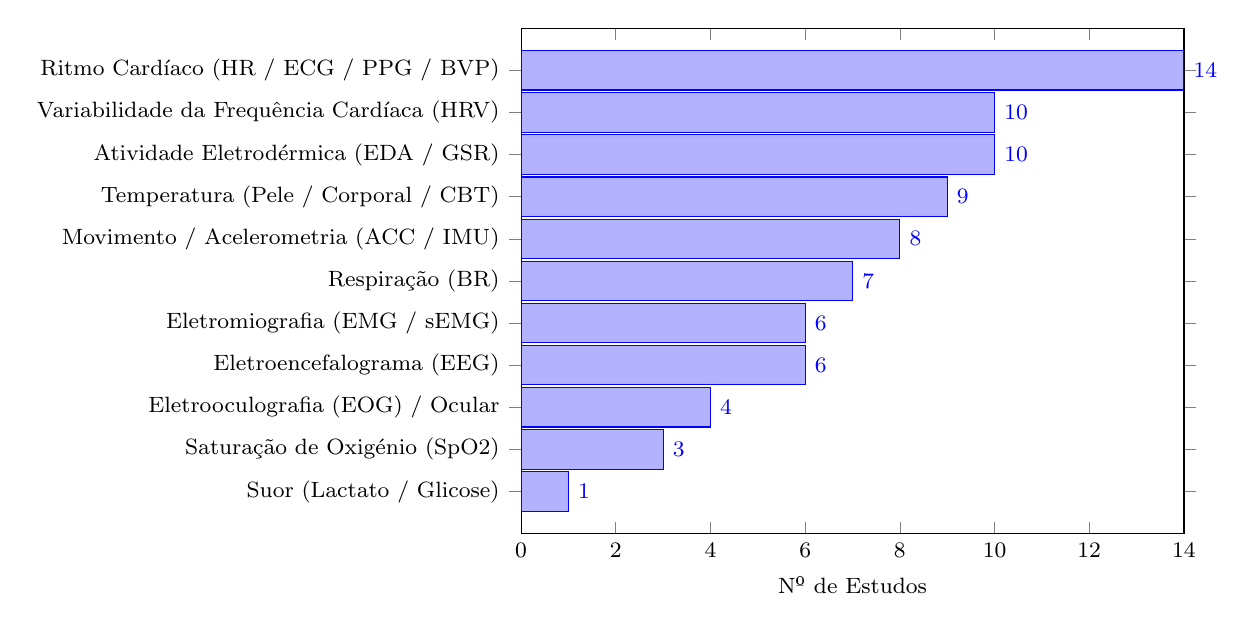
\begin{tikzpicture}
\begin{axis}[
    xbar,
    width=10cm,
    height=8cm,
    font=\footnotesize,
    xlabel={Nº de Estudos},
    ytick={1,2,3,4,5,6,7,8,9,10,11},
    yticklabels={Suor (Lactato / Glicose),Saturação de Oxigénio (SpO2),Eletrooculografia (EOG) / Ocular,Eletroencefalograma (EEG),Eletromiografia (EMG / sEMG),Respiração (BR),Movimento / Acelerometria (ACC / IMU),Temperatura (Pele / Corporal / CBT),Atividade Eletrodérmica (EDA / GSR),Variabilidade da Frequência Cardíaca (HRV),Ritmo Cardíaco (HR / ECG / PPG / BVP)},
    yticklabel style={rotate=0,anchor=east},
    nodes near coords,
    enlarge y limits=0.1,
    bar width=0.5cm,
    xmin=0,
    xmax=14,
]
\addplot coordinates {(1,1) (3,2) (4,3) (6,4) (6,5) (7,6) (8,7) (9,8) (10,9) (10,10) (14,11)};
\end{axis}
\end{tikzpicture}
\caption{Frequência de utilização de sinais fisiológicos}
\label{fig:sinais}
\end{figure}

A Figura \ref{fig:sinais} apresenta a distribuição e frequência dos sinais fisiológicos identificados no núcleo central de 14 estudos analisados nesta revisão, evidenciando as métricas utilizadas para diagnosticar estados como cansaço, fadiga ou stress. Como se pode observar, o Ritmo Cardíaco (14/14) assume-se como o sinal mais universal, sendo o indicador primário para a deteção de esforço físico e carga de trabalho, além de ser fundamental na avaliação de riscos como o stress térmico e quedas. Complementarmente, a Variabilidade da Frequência Cardíaca (HRV) (10/14) é utilizada para uma análise mais sensível, sendo crucial na transição entre estados de alerta e fadiga cognitiva ou stress mental.

A Atividade Eletrodérmica (EDA/GSR) (10/14) e a Temperatura (9/14) surgem como pilares na monitorização do stress psicológico e do esgotamento por calor, respetivamente, permitindo uma visão direta da ativação do sistema nervoso simpático e da carga térmica em ambientes industriais. No que respeita à contextualização física, o Movimento e Acelerometria (8/14) desempenha um papel duplo: identifica a intensidade da atividade e auxilia na filtragem de artefactos em sinais como PPG ou EDA.

Sinais mais específicos, como a Respiração (7/14) e a Eletromiografia (EMG) (6/14), são aplicados para medir o esforço metabólico e a fadiga muscular localizada em tarefas de manipulação manual. Por fim, a avaliação direta do estado mental e da vigilância é suportada pelo Eletroencefalograma (EEG) (6/14) e por Métricas Oculares (4/14), que permitem classificar o risco de acidentes baseados na carga cognitiva e na sonolência do trabalhador. Outras métricas, como a Saturação de Oxigénio (SpO2) (3/14) e os Biomarcadores no Suor, embora menos frequentes, oferecem uma compreensão molecular e metabólica detalhada da fadiga em condições extremas.

\subsection*{QS2: Que técnicas de aprendizagem automática e aprendizagem profunda são aplicadas para a análise e a previsão de estados humanos?}
\label{subsec:qs2}

A literatura analisada demonstra uma convergência para o uso da Inteligência Artificial (IA) como motor principal para a interpretação de dados fisiológicos. As técnicas reportadas dividem-se principalmente em duas grandes vertentes: a Aprendizagem Automática (ML) clássica para ambientes com recursos computacionais limitados e a Aprendizagem Profunda (DL) para o tratamento de sinais temporais complexos.

Dentro da Aprendizagem Automática clássica, existe um consenso sobre a eficácia dos algoritmos baseados em conjuntos (ensembles). Thomas et al. (2025) e D. Goutham et al. (2025)\cite{thomas2025,goutham2025} destacam o algoritmo XGBoost como uma das ferramentas mais potentes para classificar níveis de stress e fadiga devido à sua elevada precisão e capacidade de tratar dados tabulares. De forma semelhante, autores como Fasoyinu et al. (2025), Wang et al. (2025) e Morillo et al. (2025)\cite{fasoyinu2025,wang2024,albarran2025} reportam o uso frequente de Bosques Aleatórios (Random Forest), Máquinas de Vectores de Suporte (SVM) e K-Nearest Neighbors (KNN), salientando a sua versatilidade na classificação de atividades e na deteção de riscos.

No âmbito da Aprendizagem Profunda (DL), a abordagem desloca-se para arquiteturas capazes de capturar dependências temporais e espaciais nos sinais. Umer et al. (2025) e Karim et al. (2025)\cite{umer2025,karim2025} enfatizam o uso de redes recorrentes como LSTM (Long Short-Term Memory), Bi-LSTM e GRU (Gated Recurrent Units) para processar fluxos contínuos de dados fisiológicos. Por outro lado, a extração automática de características é abordada mediante Redes Neuronais Convolucionais (CNN), como o propõem Anjum et al. (2025) com o seu modelo personalizado FatigueNet e Ojha et al. (2024)\cite{anjum2025,ojha2024} através do uso de 1D-CNN em arquiteturas autoencoder.

Paralelamente aos métodos supervisionados, a literatura recente evidencia a adoção de técnicas de aprendizagem não supervisionada, como o \textit{clustering} e a redução de dimensionalidade (PCA), para estruturar dados fisiológicos sem etiquetas prévias. Algoritmos como o K-Means, os Modelos de Mistura Gaussiana (GMM), o DBSCAN e o \textit{Clustering} Hierárquico têm sido fundamentais para descobrir agrupamentos naturais associados ao stress e a respostas autónomas. Por exemplo, Georgiev et al. (2026)\cite{georgiev2026} destacam a utilidade do GMM para agrupar de forma exploratória respostas psicofisiológicas, enquanto Georgieva-Tsaneva et al. (2025)\cite{georgieva2025} aplicam abordagens não supervisionadas no reconhecimento de estados através da variabilidade da frequência cardíaca (HRV). Frequentemente, o \textit{clustering} atua como um passo preparatório: Messaoud et al. (2025)\cite{messaoud2025} utilizam o K-Means para categorizar padrões de HRV, usando depois essas categorizações para treinar modelos supervisionados que preveem o risco de quedas. Finalmente, no contexto da monitorização contínua, o DBSCAN destaca-se pela sua robustez; autores como Arifin et al. (2025)\cite{arifin2025} e Georgieva-Tsaneva et al. (2025)\cite{georgieva2025} utilizam-no não só para classificar atividades, mas também para identificar anomalias em tempo real e filtrar artefactos nos sensores.

Recentemente, a literatura começou a explorar modelos híbridos e técnicas avançadas para melhorar a robustez das previsões. Cheng et al. (2025) introduzem o uso de Redes Neuronais de Gráficos (GNN) para modelar variáveis dependentes do tempo, optimizadas mediante algoritmos metaheurísticos\cite{cheng2025}. Da mesma forma, Kakhi et al. (2025) e Ojha et al. (2025)\cite{kakhi2025,ojha2024} salientam o valor emergente da Aprendizagem por Transferência (Transfer Learning) e a adaptação de domínio, técnicas que permitem ajustar modelos pré-treinados à variabilidade individual de cada sujeito, superando assim uma das maiores barreiras na monitorização humana: a diferença nas respostas fisiológicas entre pessoas.

Finalmente, destaca-se a integração da Lógica Difusa (Fuzzy Logic), utilizada por Morillo et al. (2025) e Kakhi et al. (2025)\cite{albarran2025,kakhi2025} não só como preditor, mas também como mecanismo de etiquetagem objetiva de estados subjetivos como a fadiga, permitindo uma transição mais suave entre níveis de risco (baixo, médio e alto) do que a classificação binária tradicional.

\begin{figure}[H]
\centering
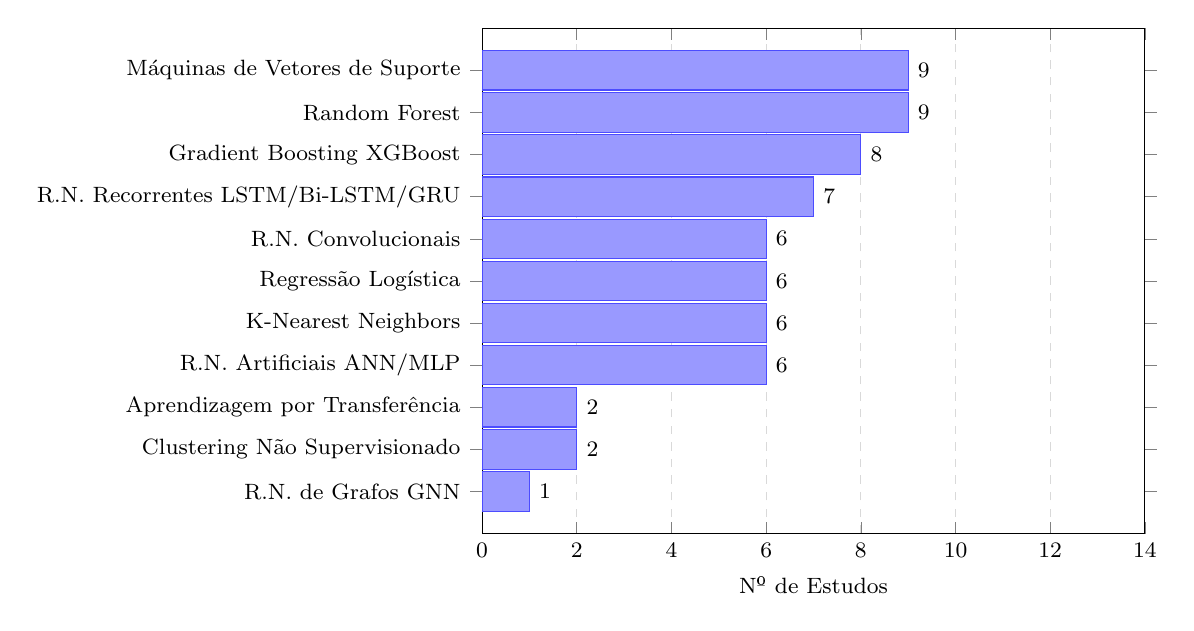
\begin{tikzpicture}
\begin{axis}[
    xbar,
    width=10cm,
    height=8cm,
    font=\footnotesize,
    xlabel={Nº de Estudos},
    symbolic y coords={
        R.N. de Grafos GNN,
        Clustering Não Supervisionado,
        Aprendizagem por Transferência,
        R.N. Artificiais ANN/MLP,
        K-Nearest Neighbors,
        Regressão Logística,
        R.N. Convolucionais,
        R.N. Recorrentes LSTM/Bi-LSTM/GRU,
        Gradient Boosting XGBoost,
        Random Forest,
        Máquinas de Vetores de Suporte
    },
    ytick=data,
    nodes near coords,
    nodes near coords align={horizontal},
    enlarge y limits=0.1,
    bar width=0.5cm,
    xmin=0,
    xmax=14, % Ajustado ao total de estudos analisados
    xmajorgrids=true,
    grid style={dashed,gray!30}
]
\addplot[fill=blue!40, draw=blue!70] coordinates {
    (1,R.N. de Grafos GNN)
    (2,Aprendizagem por Transferência)
    (6,R.N. Artificiais ANN/MLP)
    (6,K-Nearest Neighbors)
    (6,Regressão Logística)
    (6,R.N. Convolucionais)
    (7,R.N. Recorrentes LSTM/Bi-LSTM/GRU)
    (8,Gradient Boosting XGBoost)
    (9,Random Forest)
    (2,Clustering Não Supervisionado)
    (9,Máquinas de Vetores de Suporte)
};
\end{axis}
\end{tikzpicture}
\caption{Frequência de utilização de técnicas de aprendizagem automática e profunda.}
\label{fig:tecnicas_ia}
\end{figure}

A Figura \ref{fig:tecnicas_ia} apresenta a distribuição das técnicas de Inteligência Artificial aplicadas na monitorização do estado humano, revelando as abordagens predominantes nos 14 estudos analisados. Observa-se uma utilização expressiva de modelos de Aprendizagem Automática (ML) clássicos, com as Máquinas de Vetores de Suporte (SVM) e Random Forest (RF) a serem reportadas em 64,3\% dos casos (9/14). A preferência por estas técnicas deve-se à sua eficácia em conjuntos de dados de alta dimensão e à sua capacidade de lidar com dados não lineares e problemas de sobreajuste (overfitting), sendo frequentemente utilizadas para estabelecer linhas de base (baselines) de desempenho. Adicionalmente, algoritmos de Gradient Boosting, como o XGBoost (8/14), destacam-se pela sua superioridade em termos de precisão e escalabilidade no processamento de dados em tempo real.

No domínio da Aprendizagem Profunda (DL), as Redes Recorrentes (LSTM, GRU) (7/14) e as Convolucionais (CNN) (6/14) desempenham um papel fundamental na análise de séries temporais fisiológicas (como ECG e EEG), permitindo capturar dependências temporais de longo prazo e extrair automaticamente características complexas da fadiga acumulada. Verifica-se ainda uma utilização relevante de Regressão Logística e KNN (6/14), valorizados pela sua simplicidade e interpretabilidade em classificações binárias de estados de stress ou fadiga.

Por último, a Aprendizagem por Transferência (Transfer Learning) (2/14) surge como uma técnica emergente para adaptar modelos pré-treinados a novos utilizadores ou ambientes com dados limitados, ajudando a superar a variabilidade entre pessoas e melhorando a precisão de modelos em condições reais de trabalho. O Clustering Não Supervisionado (2/14) é utilizado como uma abordagem exploratória para identificar agrupamentos naturais nos dados fisiológicos, sem depender de rótulos previamente definidos, permitindo distinguir diferentes padrões ou estados fisiológicos. Adicionalmente, as Redes Neuronais de Grafos (GNN) (1/14) são aplicadas em abordagens híbridas para capturar relações complexas entre dados que mudam no tempo, como o ritmo cardíaco, e dados estáticos, sendo utilizadas especificamente para melhorar a classificação de riscos de quedas e estados de fadiga.

\subsection*{QS3: Que arquiteturas e modelos são utilizados para a análise de séries temporais fisiológicas e quais são as suas principais vantagens e limitações?}
\label{subsec:qs3}

A análise de séries temporais fisiológicas requer arquiteturas capazes de gerir a natureza sequencial e dinâmica dos dados. Segundo a literatura consultada, as arquiteturas de Redes Neuronais Recorrentes (RNN), especificamente as variantes LSTM (Long Short-Term Memory) e GRU (Gated Recurrent Units), são as mais difundidas. Umer et al. (2025) e Fasoyinu et al. (2025)\cite{umer2025,fasoyinu2025} destacam que estas redes são ideais para superar o problema do desaparecimento do gradiente, permitindo reter informação de longo prazo. Em particular, a arquitetura Bi-LSTM é assinalada por Wang et al. (2024) e Karim et al. (2025)\cite{wang2024,karim2025} como a mais precisa (atingindo até 98.5\% de exatidão), uma vez que processa a informação em ambas as direções temporais, capturando um contexto completo do sinal.

Por outro lado, o uso de Redes Neuronais Convolucionais (CNN) adaptou-se para identificar padrões espaciais e morfológicos nos sinais. Anjum et al. (2025) \cite{anjum2025} propõem FatigueNet, uma CNN concebida para lidar com a complexidade de dados heterogéneos sem o sobreajuste típico de modelos mais simples. Da mesma forma, abordagens híbridas mais recentes, como o modelo SOS-NN-GNN apresentado por Cheng et al. (2025) \cite{cheng2025}, demonstram que as Redes de Gráficos (GNN) podem superar as LSTM ao capturar dependências espaço-temporais mais complexas, integrando dados estáticos e sequenciais de forma simultânea. Especificamente, esta arquitetura combina uma Rede Neuronal (NN) para processar variáveis estáticas, uma Rede Neuronal de Gráficos (GNN) para analisar dados sequenciais e relacionais, e o algoritmo de Pesquisa de Organismos Simbióticos (SOS) para otimizar automaticamente os pesos e a estrutura do modelo. Segundo os autores, esta integração permite processar simultaneamente dados estáticos e sequenciais de forma muito mais eficaz do que os modelos tradicionais.

Quanto às vantagens, a literatura destaca a eficiência e a interpretabilidade. Modelos baseados em árvores como XGBoost e LightGBM são elogiados por D. Goutham et al. (2025) e Thomas et al. (2025)\cite{goutham2025,thomas2025} pela sua escalabilidade e rapidez, sendo LightGBM o candidato preferido para aplicações em tempo real devido ao seu baixo consumo de memória. Adicionalmente, Sim et al. (2023) \cite{sim2023} sublinham que a migração destas arquiteturas para o processamento na borda (edge computing) mediante modelos quantizados permite reduzir a latência significativamente e proteger a privacidade do utilizador.

No entanto, identificam-se limitações críticas. O desafio da "caixa negra" ou falta de interpretabilidade é uma preocupação constante para Kakhi et al. (2025) e Ojha et al. (2024)\cite{kakhi2025,ojha2024}, que argumentam que a complexidade das redes profundas dificulta a validação clínica das suas decisões. Além disso, existe uma sensibilidade inerente aos artefactos de movimento em sinais como EMG e ECG durante tarefas físicas intensas (Wang et al., 2024)\cite{wang2024}. Finalmente, Morillo et al. (2025) e Anjum et al. (2025)\cite{albarran2025,anjum2025} alertam para a baixa capacidade de \textbf{generalização} dos modelos quando se transferem de ambientes controlados de laboratório para a variabilidade extrema dos locais de obra reais, um problema que modelos como EnsmTrBoost tentam mitigar mediante a aprendizagem por transferência.

\subsection*{QS4: Quais são as métricas de avaliação mais utilizadas para validar o desempenho dos modelos propostos?}
\label{subsec:qs4}

A validação do desempenho dos modelos de inteligência artificial no âmbito da monitorização fisiológica apoia-se num conjunto diverso de métricas que permitem medir a eficácia desde distintas dimensões. De forma unânime, todos os estudos consultados, incluindo os de Fasoyinu et al. (2025), Wang et al. (2024) e Cheng et al. (2025)\cite{fasoyinu2025,wang2024,cheng2025}, reportam a Exatidão (Accuracy) como a métrica base para determinar a percentagem de previsões corretas. No entanto, dado que os dados fisiológicos frequentemente apresentam um desequilíbrio de classes (por exemplo, mais dados de "estado normal" do que de "fadiga crítica"), a literatura atribui um peso significativo à Pontuação F1 (F1-score) e à Área sob a Curva (AUC-ROC).

Autores como D. Goutham et al. (2025) e Morillo et al. (2025)\cite{goutham2025,albarran2025} priorizam o uso do F1-score e do Recall (Sensibilidade) para assegurar que o sistema não ignore estados críticos, como a fadiga severa ou o stress agudo, o que é vital para a segurança do trabalhador. Em particular, Morillo et al. (2025) \cite{albarran2025} empregam a pontuação F1 ponderada juntamente com intervalos de confiança de 95\% obtidos mediante bootstrapping para robustecer a validade estatística dos seus achados. Por sua parte, Umer et al. (2025) e Anjum et al. (2025)\cite{umer2025,anjum2025} complementam esta análise com o uso de matrizes de confusão, as quais permitem visualizar de forma detalhada os erros de classificação entre diferentes níveis de fadiga.

Em contextos onde a monitorização é abordada como um problema de previsão contínua e não apenas de classificação, utilizam-se métricas de erro de regressão. Karim et al. (2025), Kakhi et al. (2025) e Fasoyinu et al. (2024)\cite{karim2025,kakhi2025,fasoyinu2025} coincidem no uso da Raiz do Erro Quadrático Médio (RMSE) e do Erro Absoluto Médio (MAE) para quantificar o desvio das previsões relativamente aos valores fisiológicos reais.

No contexto da aprendizagem não supervisionada, a avaliação do desempenho exige métricas específicas focadas na estrutura dos agrupamentos (\textit{clusters}). Para estimar o número ideal de clústeres, Messaoud et al. (2025)\cite{messaoud2025} e Georgiev et al. (2026)\cite{georgiev2026} recorrem ao Método do Cotovelo (Elbow Method), analisando a Soma dos Erros ao Quadrado (SSE). Adicionalmente, Georgiev et al. complementam esta otimização com o Critério de Informação de Akaike (AIC) e o Critério de Informação Bayesiano (BIC). Para a validação interna, que mede a coesão e a separação espacial dos grupos, tanto Messaoud et al. como Georgieva-Tsaneva et al. (2025)\cite{georgieva2025} destacam a eficácia do Coeficiente de Silhueta (Silhouette Score), enquanto Georgieva-Tsaneva et al. utilizam também o gráfico de distância K (\textit{k-distance graph}) para calibrar a densidade no algoritmo DBSCAN. 

Finalmente, estudos com abordagens metodológicas mais avançadas introduzem métricas de consistência e similitude estatística. Ojha et al. (2024)\cite{ojha2024} destacam o uso da Divergência de Kullback-Leibler (KL) para avaliar as diferenças nas distribuições dos dados entre distintos sujeitos, assim como o desvio padrão da exatidão para medir a estabilidade do modelo perante novos utilizadores. Esta abordagem é crucial para validar a capacidade de generalização dos sistemas de monitorização em ambientes reais altamente variáveis.

\subsection*{QS5: Que limitações e desafios são identificados na literatura para a implementação de sistemas de previsão do estado humano em tempo real?}
\label{subsec:qs5}

A transição de modelos de laboratório para aplicações industriais em tempo real apresenta desafios significativos que a literatura classifica em três dimensões principais: técnica, operativa e ética.

Na dimensão técnica e operativa, existe um consenso entre autores como Wang et al. (2024) e Kakhi et al. (2025)\cite{wang2024,kakhi2025} sobre a latência na transmissão de dados para a nuvem e a instabilidade das redes em ambientes de obra. Investigações como as de Sim et al. (2023) e Umer et al. (2025)\cite{sim2023,umer2025} salientam que, embora o edge computing seja uma solução promissora, os dispositivos portáteis possuem limitações críticas de memória, capacidade de processamento e, sobretudo, vida útil da bateria. Além disso, Fasoyinu et al. (2025)\cite{fasoyinu2025} alerta para a fragilidade do hardware perante condições ambientais hostis como o pó, a humidade e a interferência electromagnética de maquinaria pesada.

Relativamente à qualidade dos dados, a literatura identifica os ``artefactos de movimento'' como a barreira principal. Ojha et al. (2024) e Wang et al. (2024)\cite{ojha2024,wang2024} explicam que atividades físicas intensas, o suor e o deslocamento dos eléctrodos geram ruído que compromete a fidelidade de sinais como o ECG e o EEG. A isto soma-se o problema da ``mudança de domínio'' (domain shift); Anjum et al. (2025) e Ojha et al. (2024)\cite{anjum2025,ojha2024} assinalam que a variabilidade fisiológica entre indivíduos (diferenças anatómicas, idade ou saúde) impede que um modelo generalizado funcione com precisão para todos os utilizadores sem um processo de calibração constante. Além disso, pessoas diferentes podem apresentar níveis de atividade física distintos, o que dificulta a criação de um único modelo capaz de classificar todos os casos, como mostram Crista, V., Martinho, D. et al. (2022)\cite{crista2022physicalactivity}.

Finalmente, os desafios humanos e éticos são determinantes para a aceitação destas tecnologias. Fasoyinu et al. (2025) e Karim et al. (2025)\cite{fasoyinu2025,karim2025} sublinham a resistência dos trabalhadores devido ao temor pela vigilância da sua produtividade e a privacidade dos seus dados biométricos e de localização. A ergonomia também desempenha um papel crucial; dispositivos volumosos ou incómodos resultam impraticáveis para jornadas laborais extensas (Wang et al., 2024)\cite{wang2024}. Por último, Umer et al. (2025) e D. Goutham et al. (2025)\cite{umer2025,goutham2025} enfatizam a falta de interpretabilidade dos modelos de aprendizagem profunda, o que gera desconfiança tanto nos utilizadores como nos responsáveis pela segurança, ao não poderem explicar o porquê de um alerta de fadiga ou stress.

\subsection*{QS6: Que mecanismos de comunicação, notificação ou retroalimentação ao utilizador são descritos na literatura?}
\label{subsec:qs6}

O sucesso dos sistemas de monitorização fisiológica não reside unicamente na precisão do diagnóstico, mas na eficácia dos seus \textbf{mecanismos de retroalimentação} para prevenir acidentes. A literatura identifica uma hierarquia de notificações que varia segundo a urgência do estado detetado e o papel do recetor (trabalhador ou supervisor).

Esta importância do feedback personalizado é também destacada por Ribeiro, R., Martinho, D. et al.~\cite{ribeiro2026wearable}, que associam mecanismos de retroalimentação adequados ao aumento do envolvimento e da adesão dos utilizadores. De forma complementar, Martinho, D. et al.~\cite{martinho2023elderlycare} apresentam um sistema com um assistente virtual que interage com o utilizador, fornece feedback personalizado sobre o seu estado de saúde e utiliza técnicas de gamificação. No contexto desta tese, os alertas devem ter em consideração o estado fisiológico, a função e os valores de referência individuais de cada trabalhador. Isto permitirá adaptar os limiares de alerta, o conteúdo das notificações e o canal utilizado para as comunicar. Por exemplo, uma alteração moderada poderá gerar uma recomendação de pausa para um trabalhador que apresente sinais de fadiga, enquanto, para outro trabalhador, a mesma alteração poderá ser considerada parte do seu esforço habitual e exigir apenas um acompanhamento contínuo.

No nível individual, as alertas hápticas e tácteis são reportadas como as mais eficazes pela sua natureza não intrusiva. Fasoyinu et al. (2024) e Wang et al. (2024)\cite{fasoyinu2025,wang2024} descrevem o uso de motores de vibração integrados em cinturões, coletes ou relógios inteligentes que alertam o operador sobre fadiga crítica ou proximidade a zonas de perigo. Esta retroalimentação complementa-se com interfaces visuais em dispositivos móveis e óculos de realidade aumentada, onde se apresentam avisos gráficos sobre o estado de saúde atual (Kakhi et al., 2025)\cite{kakhi2025}.

Por outro lado, autores como Thomas et al. (2025)\cite{thomas2025} e Ojha et al. (2024)\cite{ojha2024} destacam a implementação de intervenções sugeridas. Em vez de emitir apenas um alerta, os sistemas baseados em IoT enviam notificações personalizadas via SMS ou aplicações móveis recomendando ações específicas, tais como realizar exercícios de respiração, tomar uma micro-pausa de recuperação ou ingerir suplementos de electrólitos perante o stress térmico. Em casos de fadiga extrema ou sonolência, Wang et al. (2024)\cite{wang2024} menciona mesmo o uso de estímulos auditivos (música) para despertar ou reanimar o utilizador.

A nível de gestão, a literatura enfatiza a importância dos painéis de controlo (dashboards) e plataformas web. Cheng et al. (2025)\cite{cheng2025} integram a monitorização com modelos BIM (Building Information Modeling) para visualizar em tempo real a localização e o nível de risco dos trabalhadores num ambiente 3D, permitindo aos engenheiros de segurança tomar decisões informadas sobre a rotação de tarefas. No entanto, Morillo et al. (2025)\cite{albarran2025} sublinham que esta comunicação para os supervisores deve ser gerida sob esquemas pseudonimizados para proteger a privacidade do trabalhador, ativando apenas protocolos de intervenção assistida quando se deteta "fadiga pura".

Finalmente, observa-se o uso da retroalimentação bidireccional. Estudos como os de Anjum et al. (2025)\cite{anjum2025}, Sim et al. (2023)\cite{sim2023} e Umer et al. (2025)\cite{umer2025} utilizam avisos (prompts) nos dispositivos portáteis para que o utilizador valide subjetivamente o seu estado mediante escalas como a Classificação de Fadiga (ROF). Este mecanismo não só serve como uma notificação de segurança, mas também atua como uma ferramenta de recalibração constante para os modelos de aprendizagem automática.

\section{Análise dos resultados}
\label{sec:analisis}

Nesta secção aprofunda-se a interpretação dos resultados apresentados na secção anterior, procurando fechar e consolidar cada pergunta desde a perspetiva desta dissertação de tese, destacando as implicações práticas, as oportunidades de melhoria e a forma como estes achados orientam o design do gémeo digital humano proposto.

\subsection{Respostas às perguntas de investigação}

\subsubsection*{QS1: Que tipos de sinais fisiológicos são mais comummente recolhidos e utilizados na literatura para a monitorização do estado humano?}
\label{subsubsec:qs1_analisis}

A análise dos resultados revela que a monitorização do estado humano em ambientes de risco assenta numa hierarquia clara de sinais, onde a frequência cardíaca (HR) e a sua variabilidade (HRV) surgem como os indicadores mais robustos e viáveis. Para os objetivos desta dissertação, este achado é fundamental, uma vez que valida a utilização de sensores wearables não intrusivos, como relógios inteligentes e bandas peitorais, que apresentam uma elevada aceitabilidade em contexto de obra. O predomínio destes sinais na literatura (14/14 estudos) confirma que as métricas cardiovasculares oferecem a sensibilidade necessária para detetar precocemente a fadiga e o stress, permitindo a criação de um sistema de alertas em tempo real que constitui o eixo central desta investigação.

Por outro lado, a literatura revista sugere que a eficácia dos modelos de IA aumenta significativamente quando se adota uma abordagem multimodal. Neste contexto, a elevada frequência de utilização da Atividade Eletrodérmica (EDA) e da Temperatura (10/14 estudos) indica que estes sinais fisiológicos são especialmente relevantes como fontes de informação complementares. Na perspetiva desta tese, a integração destes sinais secundários, disponíveis em sensores modernos, representa uma oportunidade para aumentar a precisão na previsão de estados críticos.

Embora sinais como a eletroencefalografia (EEG) ou a eletromiografia (EMG) ofereçam dados detalhados, a sua baixa adoção em ambientes industriais (devido à sua intrusividade e à sensibilidade ao ruído de movimento) reforça a decisão desta investigação de se focar em dados sequenciais provenientes de dispositivos portáteis.

Em suma, os achados orientam o design do gémeo digital proposto para uma arquitetura que prioriza sinais cardiovasculares e térmicos, complementados por medidas auxiliares como a acelerometria e a respiração, garantindo assim um equilíbrio entre o rigor científico do diagnóstico e a viabilidade prática da monitorização contínua em trabalhos de alto risco.

\subsubsection*{QS2: Que técnicas de aprendizagem automática e aprendizagem profunda são aplicadas com maior frequência para a análise e a previsão de estados como stress, fadiga, carga fisiológica ou nível de atenção?}
\label{subsubsec:qs2_analisis}

A convergência da literatura para modelos de IA demonstra que a complexidade dos sinais fisiológicos recolhidos por wearables exige algoritmos que superem as análises estatísticas tradicionais, embora não requeiram necessariamente modelos de aprendizagem profunda em todos os cenários. No contexto desta tese, a elevada prevalência de modelos clássicos como as Máquinas de Vetores de Suporte (SVM) e Random Forest (9/14 estudos) constitui um indicador crítico. Estes modelos são adequados para a implementação em dispositivos com recursos computacionais limitados, sugerindo que o gémeo digital proposto pode integrar classificadores robustos que garantam respostas rápidas em ambientes de obra, onde a latência na deteção de um estado crítico pode comprometer a segurança do trabalhador.

Por outro lado, a tendência para o uso de Aprendizagem Profunda (DL), especificamente redes LSTM e GRU, justifica a necessidade de tratar os dados dos sensores (frequência cardíaca e temperatura) como séries temporais contínuas e não como eventos isolados. Dado que esta investigação tem como objetivo prever a fadiga e o stress (estados que se acumulam ao longo do tempo), a capacidade destas redes para reter informação de longo prazo revela-se fundamental. A análise sugere que uma arquitetura híbrida, que combine a extração de características de modelos convolucionais com a memória temporal das redes recorrentes, poderá oferecer o equilíbrio necessário entre precisão diagnóstica e fiabilidade nas alertas.

Finalmente, a identificação na literatura de técnicas como a Aprendizagem por Transferência (Transfer Learning), o Clustering Não Supervisionado e a Lógica Difusa orienta esta dissertação para a resolução de três problemas práticos: a variabilidade biológica entre trabalhadores, a descoberta de padrões fisiológicos sem etiquetas prévias e a subjetividade dos estados de fadiga. A integração de lógica difusa permite que o sistema de alertas não seja apenas binário, mas que possa comunicar níveis de risco progressivos (baixo, moderado, elevado), o que é significativamente mais útil para a gestão de segurança em obra do que um simples estado de 'fadiga/não fadiga'. O clustering pode ainda funcionar como uma etapa exploratória e de preparação dos dados, contribuindo para identificar padrões naturais antes da aplicação de modelos preditivos. Em conclusão, os resultados apontam para um design de software que prioriza a robustez do machine learning clássico para o processamento imediato, a exploração não supervisionada dos dados e a profundidade do deep learning para a análise preditiva da evolução do estado do trabalhador.

\subsubsection*{QS3: Que arquiteturas e modelos são utilizados para a análise de séries temporais fisiológicas e quais são as suas principais vantagens e limitações?}
\label{subsubsec:qs3_analisis}

A análise da literatura revela que a monitorização eficaz dos estados humanos não depende unicamente da escolha do algoritmo, mas também da sua capacidade para lidar com a natureza sequencial dos dados fisiológicos. Para os objetivos desta tese, a relevância das arquiteturas LSTM e Bi-LSTM constitui uma conclusão determinante. Estas redes recorrentes de aprendizagem profunda são essenciais para captar a memória temporal do sinal, permitindo ao sistema distinguir entre um esforço físico momentâneo e uma tendência de fadiga acumulada ao longo de várias horas.

Por outro lado, a literatura destaca as vantagens dos modelos de aprendizagem automática baseados em árvores, como o LightGBM. Embora este algoritmo tenha sido concebido para dados tabulares, a sua aplicação a séries temporais é possível através da extração de características (\textit{feature extraction}), convertendo segmentos de sinais sequenciais em métricas estatísticas. Esta abordagem permite aproveitar a rapidez e o baixo consumo de memória do LightGBM, reforçando a viabilidade do Edge Computing. No contexto desta tese, isto significa que o processamento pode ocorrer localmente no dispositivo móvel ou wearable, garantindo respostas rápidas e a privacidade do trabalhador sem a necessidade de uma ligação constante à nuvem nos estaleiros.

Por fim, as limitações reportadas na literatura têm implicações diretas no desenho desta tese. Primeiro, a sensibilidade ao movimento significa que o sistema pode confundir sinais fracos ou distorcidos pelo movimento do trabalhador com sinais de fadiga; por isso, esta investigação dará prioridade a técnicas de filtragem de dados. Isto realça a importância de incluir uma camada prévia de limpeza e preparação dos dados antes de os submeter aos modelos, assegurando que apenas se processem sinais fisiológicos relevantes e reduzindo a possibilidade de falsos alertas. Segundo, a baixa capacidade de generalização indica que os modelos treinados em laboratório falham frequentemente em ambientes de obra reais. Para mitigar este problema, o Gémeo Digital proposto irá focar-se na robustez dos dados, utilizando dados reais de trabalhadores de obra para o treino dos modelos, assegurando que os alertas de segurança sejam fiáveis e baseados em variações fisiológicas reais.

\subsubsection*{QS4: Quais são as métricas de avaliação mais utilizadas para validar o desempenho dos modelos propostos em estudos de monitorização fisiológica?}
\label{subsubsec:qs4_analisis}

O análise das métricas de avaliação revela que a eficácia de um Gémeo Digital para a segurança laboral não pode ser medida apenas pela Exactidão (Accuracy). Embora esta métrica seja a mais comum, a literatura alerta para o problema do desequilíbrio de classes nos dados fisiológicos, onde os estados de risco (fadiga severa ou stress agudo) são menos frequentes do que o estado normal. Para os objetivos desta tese, esta descoberta é crucial: o sistema de alertas deve ser validado prioritariamente através do F1-score e do Recall (Sensibilidade). Na perspetiva da segurança em obra, um valor elevado de Recall garante que o modelo minimize os falsos negativos, assegurando que nenhum estado de perigo real passe despercebido, o que é vital para a prevenção de acidentes.

Além disso, a inclusão de métricas de regressão como o MAE (Erro Absoluto Médio) e o RMSE (Root Mean Squared Error / Raiz do Erro Quadrático Médio) na literatura orienta o desenho desta investigação para uma monitorização proativa. Em vez de apenas classificar se o trabalhador “está ou não” fatigado, o uso destas métricas permite avaliar a precisão do sistema ao prever a tendência de evolução dos sinais vitais. Isto possibilita que o Gémeo Digital antecipe estados críticos antes de estes atingirem limiares perigosos.

Na aprendizagem não supervisionada, a avaliação exige métricas centradas na estrutura dos agrupamentos. O Método do Cotovelo (Elbow Method) estima o número adequado de clústeres através da Soma dos Erros ao Quadrado (SSE). Este procedimento pode ser complementado pelo Critério de Informação Bayesiano (BIC), que seleciona o modelo equilibrando a qualidade do ajuste e a complexidade. Após a definição dos agrupamentos, o Coeficiente de Silhueta (Silhouette Score) avalia a coesão interna e a separação entre grupos. Em conjunto, estas métricas permitem verificar se os padrões fisiológicos são consistentes, interpretáveis e úteis para detetar estados de stress e fadiga.

Por último, o uso da Divergência de Kullback-Leibler (KL) e do desvio padrão da exactidão, mencionados em estudos mais recentes, reforça a necessidade de testar a estabilidade do modelo entre diferentes indivíduos. A KL permite avaliar quanto se diferenciam os padrões fisiológicos de cada trabalhador relativamente aos dados médios do modelo, assegurando que o sistema seja capaz de se adaptar a diferentes variações individuais e não falhe com pessoas cujos sinais sejam pouco comuns. Por sua vez, o desvio padrão mede a consistência do modelo entre diferentes trabalhadores. Assim, a validação não se centra apenas na média de desempenho, mas na capacidade do modelo de manter resultados fiáveis e consistentes face à variabilidade individual, garantindo que o Gémeo Digital seja uma ferramenta de segurança robusta e não apenas um modelo estatístico de laboratório.

\subsubsection*{QS5: Que limitações e desafios são identificados na literatura para a implementação de sistemas de previsão do estado humano em tempo real?}
\label{subsubsec:qs5_analisis}

A transposição das métricas de laboratório para o ambiente operativo de uma obra exige que o sistema desenhado nesta investigação possua uma arquitetura resiliente face a falhas de infraestrutura. Perante a instabilidade da rede e os problemas de latência reportados, esta tese propõe uma estratégia de computação descentralizada. Ao processar os algoritmos de deteção de fadiga localmente (edge computing), o Gémeo Digital garante que os alertas de segurança sejam disparados instantaneamente, limitando a dependência total de uma ligação estável à nuvem. Esta escolha técnica também resolve a limitação da duração da bateria, ao reduzir a frequência de transmissões de dados sem fios de alto consumo.

No que respeita à integridade dos dados em ambientes hostis, esta investigação aborda a fragilidade dos sensores através da utilização combinada de relógios inteligentes e bandas torácicas. Esta abordagem multimodal é estratégica: enquanto o relógio oferece versatilidade e sinais complementares (como temperatura e acelerometria), a banda torácica assegura uma medição do ritmo cardíaco mais precisa e menos vulnerável aos artefactos de movimento do que os sensores apenas de pulso. As fraquezas dos relógios são compensadas pela precisão das bandas torácicas e, por sua vez, as limitações destas últimas são equilibradas com a informação adicional fornecida pelos relógios. Adicionalmente, para abordar o problema da variabilidade fisiológica individual, poderia ser integrado um processo de calibração adaptativa no Gémeo Digital. Isto permitiria ajustar os limiares de alerta ao perfil base de cada trabalhador, transformando o desafio da generalização numa oportunidade para personalizar a segurança.

\subsubsection*{QS6: Que mecanismos de comunicação, notificação ou retroalimentação ao utilizador são descritos na literatura?}
\label{subsubsec:qs6_analisis}

A análise dos mecanismos de comunicação sugere caminhos promissores para a interação entre o Gémeo Digital e o utilizador, procurando que a comunicação seja clara e gerível. Para esta tese, pode colocar-se a hipótese de explorar alertas hápticas (vibração) como canal prioritário. Num ambiente de obra, onde o ruído ambiental é elevado e a atenção visual é crítica para a tarefa, faz sentido considerar a vibração no relógio inteligente e na banda torácica como uma possibilidade menos intrusiva e potencialmente mais eficaz para notificações de fadiga ou stress.

Adicionalmente, existe a possibilidade de incorporar mecanismos de retroalimentação bidireccional. Este conceito permitiria que o trabalhador validasse subjetivamente o seu estado através do dispositivo, funcionando não apenas como um alerta, mas como uma ferramenta potencial para o ajuste e refinamento contínuo dos modelos de aprendizagem automática com base no feedback real do utilizador.

Por último, a literatura indica que a integração de camadas de informação visual ou dashboards constitui uma vantagem para a gestão da segurança. Pode considerar-se a inclusão de interfaces que apresentem níveis de risco processados, permitindo uma visualização clara dos estados críticos sem comprometer a privacidade dos dados fisiológicos brutos. Em suma, estas opções de comunicação e visualização representam caminhos a explorar no desenho do Gémeo Digital, com o objetivo de encontrar o equilíbrio ideal entre a prontidão da resposta e a viabilidade operacional no terreno.

\subsection{Conclusões}
\label{subsec:conclusiones}

A análise detalhada das questões de investigação permite concluir que o desenvolvimento de um Gémeo Digital Humano para a segurança na construção civil exige equilibrar a precisão de laboratório com a fiabilidade em condições reais. Os achados revistos indicam que uma arquitetura baseada em sensores não intrusivos (relógios e bandas torácicas) permite monitorizar continuamente indicadores de fadiga e stress de forma fiável para o trabalhador, evitando depender de sinais intrusivos e priorizando a robustez dos dispositivos wearables.

Além disso, a combinação de modelos híbridos de aprendizagem automática e processamento local (Edge Computing) surge como uma estratégia chave para garantir alertas imediatos e mitigar problemas de conectividade. Mais do que a simples exatidão, a atenção ao Recall e ao F1-score nas métricas de avaliação sublinha que o sucesso deste Gémeo Digital se medirá pela sua capacidade de não ignorar estados de risco, priorizando a salvaguarda da vida humana.

Por fim, a personalização mediante calibrações adaptativas e a utilização de alertas hápticos ou visuais identificam-se como mecanismos críticos para superar a variabilidade individual e o ruído ambiental. Em conjunto, estes achados fornecem as bases teóricas e técnicas que orientam o desenho do Gémeo Digital como uma ferramenta de segurança proativa, fiável e sustentável em ambientes reais de risco.